
\documentclass[xcolor=svgnames]{beamer}

\usepackage[utf8]    {inputenc}
\usepackage[T1]      {fontenc}
\usepackage[english] {babel}

\usepackage{amsmath,amsfonts,graphicx}
\usepackage{beamerleanprogress}
\usepackage{tikz}
\usepackage{fancyvrb}
\usepackage{listings} 
\usepackage{multicol}
\usepackage{pifont}
\usepackage{hyperref}
\hypersetup{
    colorlinks=true,
    linkcolor=blue,
    filecolor=magenta,      
    urlcolor=cyan,
}

% for straight apostrophe
\makeatletter
\let \@sverbatim \@verbatim
\def \@verbatim {\@sverbatim \verbatimplus}
{\catcode`'=13 \gdef \verbatimplus{\catcode`'=13 \chardef '=13 }} 
\makeatother

\definecolor{iyellow}{RGB}{255, 162, 23}
\definecolor{sgreen}{RGB}{118, 191, 138}

\newcommand{\yellow}[1]{\textcolor{iyellow}{#1}}
\newcommand{\red}[1]{\textcolor{red}{#1}}
\newcommand{\green}[1]{\textcolor{ForestGreen}{#1}}
\newcommand{\blue}[1]{{\textcolor{blue}{#1}}}
\newcommand{\orange}[1]{{\textcolor{orange}{#1}}}
\newcommand{\bblue}[1]{\textcolor{SteelBlue!90!gray}{#1}} % beamer blue
\newcommand{\purple}[1]{{\textcolor{purple}{#1}}}

\newcommand{\el}{\\[1em]\pause}
\newcommand{\nl}{\\[1em]}
\newcommand{\define}[1]{\textbf{\textcolor{orange}{#1}}}

%\newcommand{\answer}[1]{\textit{\textbf{\textcolor{iyellow}{#1}}}}

\newcommand{\command}[1]{\texttt{\textbf{\textcolor{DarkMagenta}{#1}}}}
\newcommand{\ipic}[2]{\includegraphics[width={#2}\textwidth]{#1}}
\newcommand{\cell}[1]{{\sf \textbf{\textcolor{DarkMagenta}{#1}}}}
\newcommand{\ra}{$\rightarrow$}

\newcommand{\ft}[1]{\frametitle{#1}}


\newenvironment{allintypewriter}{\ttfamily}{\par}
\newcommand{\bs}{$\backslash$}

\newcommand*\keystroke[1]{%
  \tikz[baseline=(key.base)]
    \node[%
      draw,
      fill=white,
      drop shadow={shadow xshift=0.25ex,shadow yshift=-0.25ex,fill=black,opacity=0.75},
      rectangle,
      rounded corners=2pt,
      inner sep=1pt,
      line width=0.5pt,
      font=\scriptsize\sffamily
    ](key) {#1\strut}
  ;
}

% timed answer
\newcommand{\tans}[2]{\textbf<#1>{\textit<#1>{{\color<#1>{iyellow}{#2}}}}}


\makeatletter
\g@addto@macro\normalsize{%
  \setlength\abovedisplayskip{0.4em}
  \setlength\belowdisplayskip{0.4em}
  \setlength\abovedisplayshortskip{0.2em}
  \setlength\belowdisplayshortskip{0.2em}
}
\makeatother


\newcommand{\cmark}{{\Large\color{green}\ding{51}}}%
\newcommand{\xmark}{{\Large\color{red}\ding{55}}}%

\newcommand{\pcmark}{\onslide<+->{\cmark}}
\newcommand{\pxmark}{\onslide<+->{\xmark}}

\newcommand{\by}{\overline{y}}
\newcommand{\ty}{\tilde{y}}

\urldef{\webmaccom}\url{https://developers.google.com/maps/documentation/geocoding/start?utm_source=google&utm_medium=cpc&utm_campaign=FY18-Q2-global-demandgen-paidsearchonnetworkhouseads-cs-maps_contactsal_saf&utm_content=text-ad-none-none-DEV_c-CRE_315916117598-ADGP_Hybrid+\%7C+AW+SEM+\%7C+BKWS+~+Google+Maps+Geocoding+API-KWID_43700039136946117-kwd-300650646186-userloc_9001467&utm_term=KW_google\%20geocoding\%20api-ST_google+geocoding+api&gclid=CO6SkMLfk-ECFcWVxQId9hsKBA} % in the preamble




\title
  [Data 301 Data Analytics\hspace{2em}]
  {Data 301 Data Analytics\\
  GIS}

\author
  [Dr.\ Irene Vrbik]
  {Dr.\ Irene Vrbik}

\date
  {Term 1, 2018}

\institute
  {University of British Columbia Okanagan \newline irene.vrbik@ubc.ca}

\graphicspath{{img/}}

\begin{document}

\maketitle

\section
  {Intro}
  
  
\begin{frame}
  {Why learn Geographic Information Systems?}
	Geographic Information Systems (GIS) are used in a wide variety of areas for the analysis and display of spatial and geographical data:

	 
\begin{columns}[T] % align columns
\begin{column}{.55\textwidth}
	\begin{itemize}
		  \item City and infrastructure planning
		  \item Business development, planning, forecasting
		  \item Store placement, sales trends
		  \item Population forecasting and analysis
		  \item Environmental and water
	  \end{itemize}
	  \end{column}%
\hfill%
\begin{column}{.48\textwidth}
 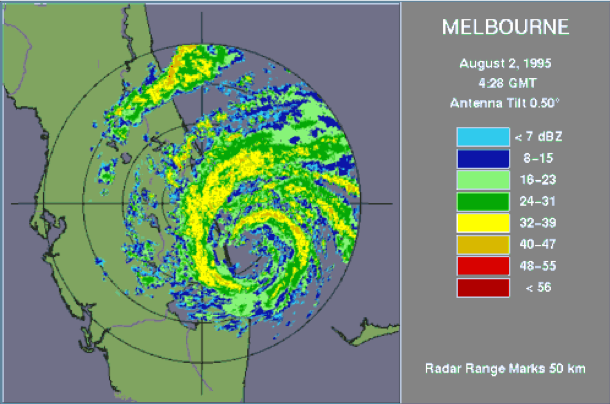
\includegraphics[width=0.9\textwidth]{GIS1}\end{column}%
\end{columns}


\end{frame}

\begin{frame}
{What is a Geographic Information System?}
\define{Geographic Information Systems} are systems designed for storing, manipulating, analyzing, and displaying spatial and geographical data.\nl

A GIS will contain components:

\begin{itemize}
\item for importing data from various sources in different formats
\item organizing the data into layers or groups
\item composing and integrating data to produce new information
\item displaying the data visually as maps or 3D visualizations to help interpret the data
\end{itemize}
\end{frame}




\begin{frame}\ft{GIS History}
\begin{itemize}
\item The technique of \emph{overlaying} information on maps dates back long before computers.\nl
\item In the 1960s geographic mapping software developed the basic GIS concepts. \nl
\item The first GIS was developed by  \href{http://www.theglobeandmail.com/report-on-business/roger-tomlinson-put-geography-on-the-map/article1461577/}{Dr. Roger Tomlinson} for Canadian Department of Forestry and Rural Development.\nl
\item Tomlinson revolutionized this discipline when he introduced GIS for scanning maps into a computer and allowing not only physical landmark data, but things like population patterns, and animal migration routes in these areas to be mapped and used for statistical analysis.% along with related statistical information about the region.
\end{itemize}

\end{frame}

\begin{frame}\ft{GIS History}

In 1969, Environmental Systems Research Institute (ESRI) founded by Laura and Jack Dangermond and developed suite of products.\nl
\begin{itemize}
\item ESRI now the de facto standard for commercial GIS products (e.g. ArcGIS, ArcView).\nl
%\item Software linked spatial representation of features with table attributes
\item The software facilitates location-based analytics and provides {contextual tools for mapping and spatial reasoning}.  Read more  \hyperlink{https://www.esri.com/en-us/arcgis/about-arcgis/overview}{here}.\nl
\end{itemize}
Listen to \href{https://www.esri.com/about/newsroom/podcast/the-power-of-design-thinking/}{this} podcast on how the combination of data, advanced analytics, and visualization of geospatial information magnifies the power of design.
\end{frame}


\begin{frame}\ft{GIS Features}
A GIS allows a user to add (or overlay) data on a map including:

\begin{description}
%\item[Annotation] (text)  name or description of item/feature (e.g. city name)
\item[Point]  a single (x,y) co-ordinate on the map
\item[Line] a connected pair of two (x,y) points
\item[Polygon] three or more (x,y) points connected to form a closed shape
\end{description}

These geometric shapes represent a \define{feature}; that is, anything you can see on the landscape. \nl

The GIS feature consists of coordinates placing it on the map.


\end{frame}

\begin{frame}\ft{GIS Data types}
%The GIS feature consists of coordinates placing it on the map.\nl
%Each feature can have attributes providing additional information.\nl
Each \emph{feature} can have one or more additional \emph{attributes} (data items) describing it.
\begin{itemize}
\item For example, a city could be represented as a point on the map (with coordinates) and additional attributes include its name and population.\nl

\end{itemize}


These attributes may have data types such as:
\begin{description}
\item[Text] for names and labels
\item[Categories] for grouping similar features/classes (road, land use, etc.)
\item[Numbers] for measurements (population, rainfall, etc.)
\end{description}
\end{frame}




\begin{frame}\ft{GIS Data types}
\begin{itemize}
\item Data is often placed in categories for display. \nl
\item Each item in the category has the same symbol.\nl

\item Measurement data is also grouped into categories to ease understanding even if the data is continuous. \nl
\begin{itemize}
%\item  For example, ordinal data has categories ranked according to a scale: low, medium, high
\item For example, elevation might be discretized into a finite number of bins in order to display this information easily on a map. 
\end{itemize}



\end{itemize}



\end{frame}

\begin{frame}\ft{GIS Interval Data}
Interval data has values along a regular numeric scale. \href{http://www12.statcan.gc.ca/census-recensement/2011/geo/map-carte/ref/thematic_download-thematiques_telecharger-eng.cfm?SERIES=B&CACODE=915&CANAME=Kelowna}{Source for image: Stats Can}
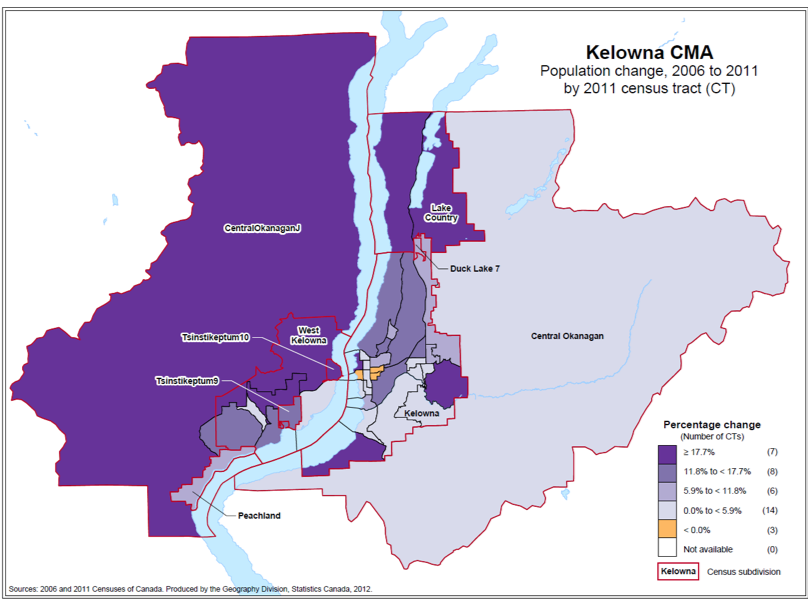
\includegraphics[height=0.55\textheight]{img/purplemap.png}
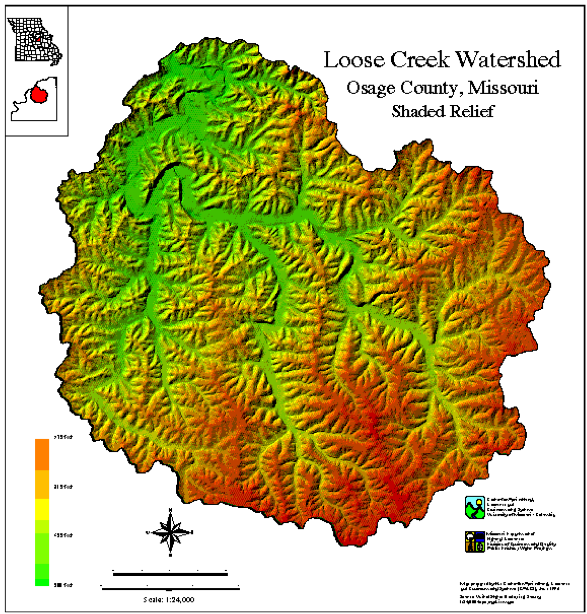
\includegraphics[height=0.55\textheight]{img/watermap.png}
\end{frame}


\begin{frame}\ft{GIS Terminology: Scale and Precision}
\begin{columns}[T] % align columns
\begin{column}{.5\textwidth}
\define{Scale} is the ratio of size on the ground to size on the map.\nl
\define{Accuracy} is a measure of how accurate the map representation is compared to the real-world.\nl
%\define{Precision} refers to the level of measurement and exactness of description in a GIS database. 
%\begin{itemize}
%\item If map symbol is 1 point (72 points=1 inch) and scale is 1:100000, then symbol S = 100,000 points = 1388 inches = 115 feet is uncertainty in placement based on representation.
%\end{itemize}
\define{Resolution} %is the sampling distance of the stored x-y values.
is the smallest difference between adjacent positions that can be recorded
\end{column}%
\hfill%
\begin{column}{.48\textwidth}
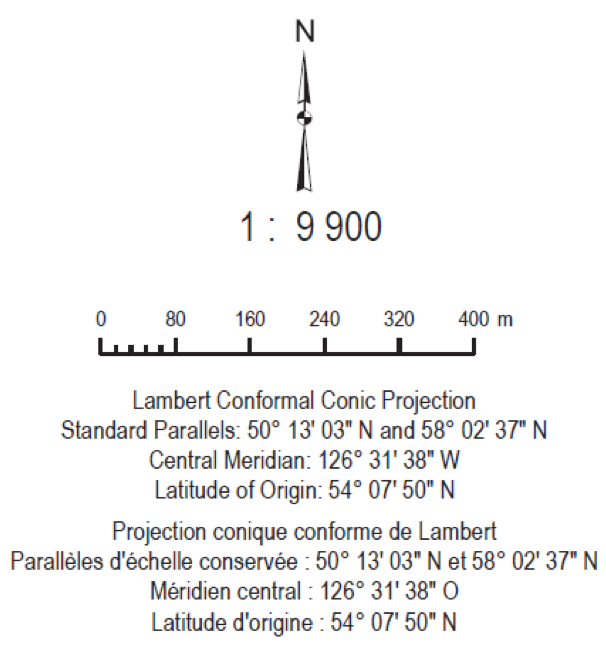
\includegraphics[width=0.9\textwidth]{img/compass.png}
\end{column}%
\end{columns}
\end{frame}

\begin{frame}
\begin{example}
 If the scale of the map is 1:100000, and the feature on the map is 3 cm long, how long is the feature in the real-world?
\begin{enumerate}[A)]
\item 1 cm	
\item 3 cm
\item 300000 m	
\item 300 m	
\item \tans{2}{3cm = 300000 cm = 3 km}
\end{enumerate}
\end{example}
\end{frame}
%
%
%\begin{frame}
%\begin{example}
% If the scale of the map is 1:100000, and a road is represented on the map by a line that is 2 mm thick, what is the error in representation (i.e. how far off can the road be in real-life)?
%\begin{enumerate}[A)]
%\item 2 km	
%\item \tans{2}{200 m}
%\item 20 m
%\item 2 m
%\item  No error
%\end{enumerate}
%\end{example}
%\end{frame}





\begin{frame}\ft{Feature Classes and Layers}
A \define{feature class} is a collection of objects with the same attributes. 
\begin{itemize}
\item May be stored as individual rows of a single table
\item Have the same geometry (e.g. all points or all polygons).
\item Example classes: states, cities, rivers.\nl
\end{itemize}

A \define{layer} is a grouping of features that can be added or removed from the map (and its display visualization).
\begin{itemize}
\item A layer will often reference or use a feature class.
\end{itemize}
\end{frame}

\begin{frame}
\ft{Kelowna}
Feature Class and Layer Screenshot \href{https://maps.kelowna.ca/public/mapviewer/}{source}
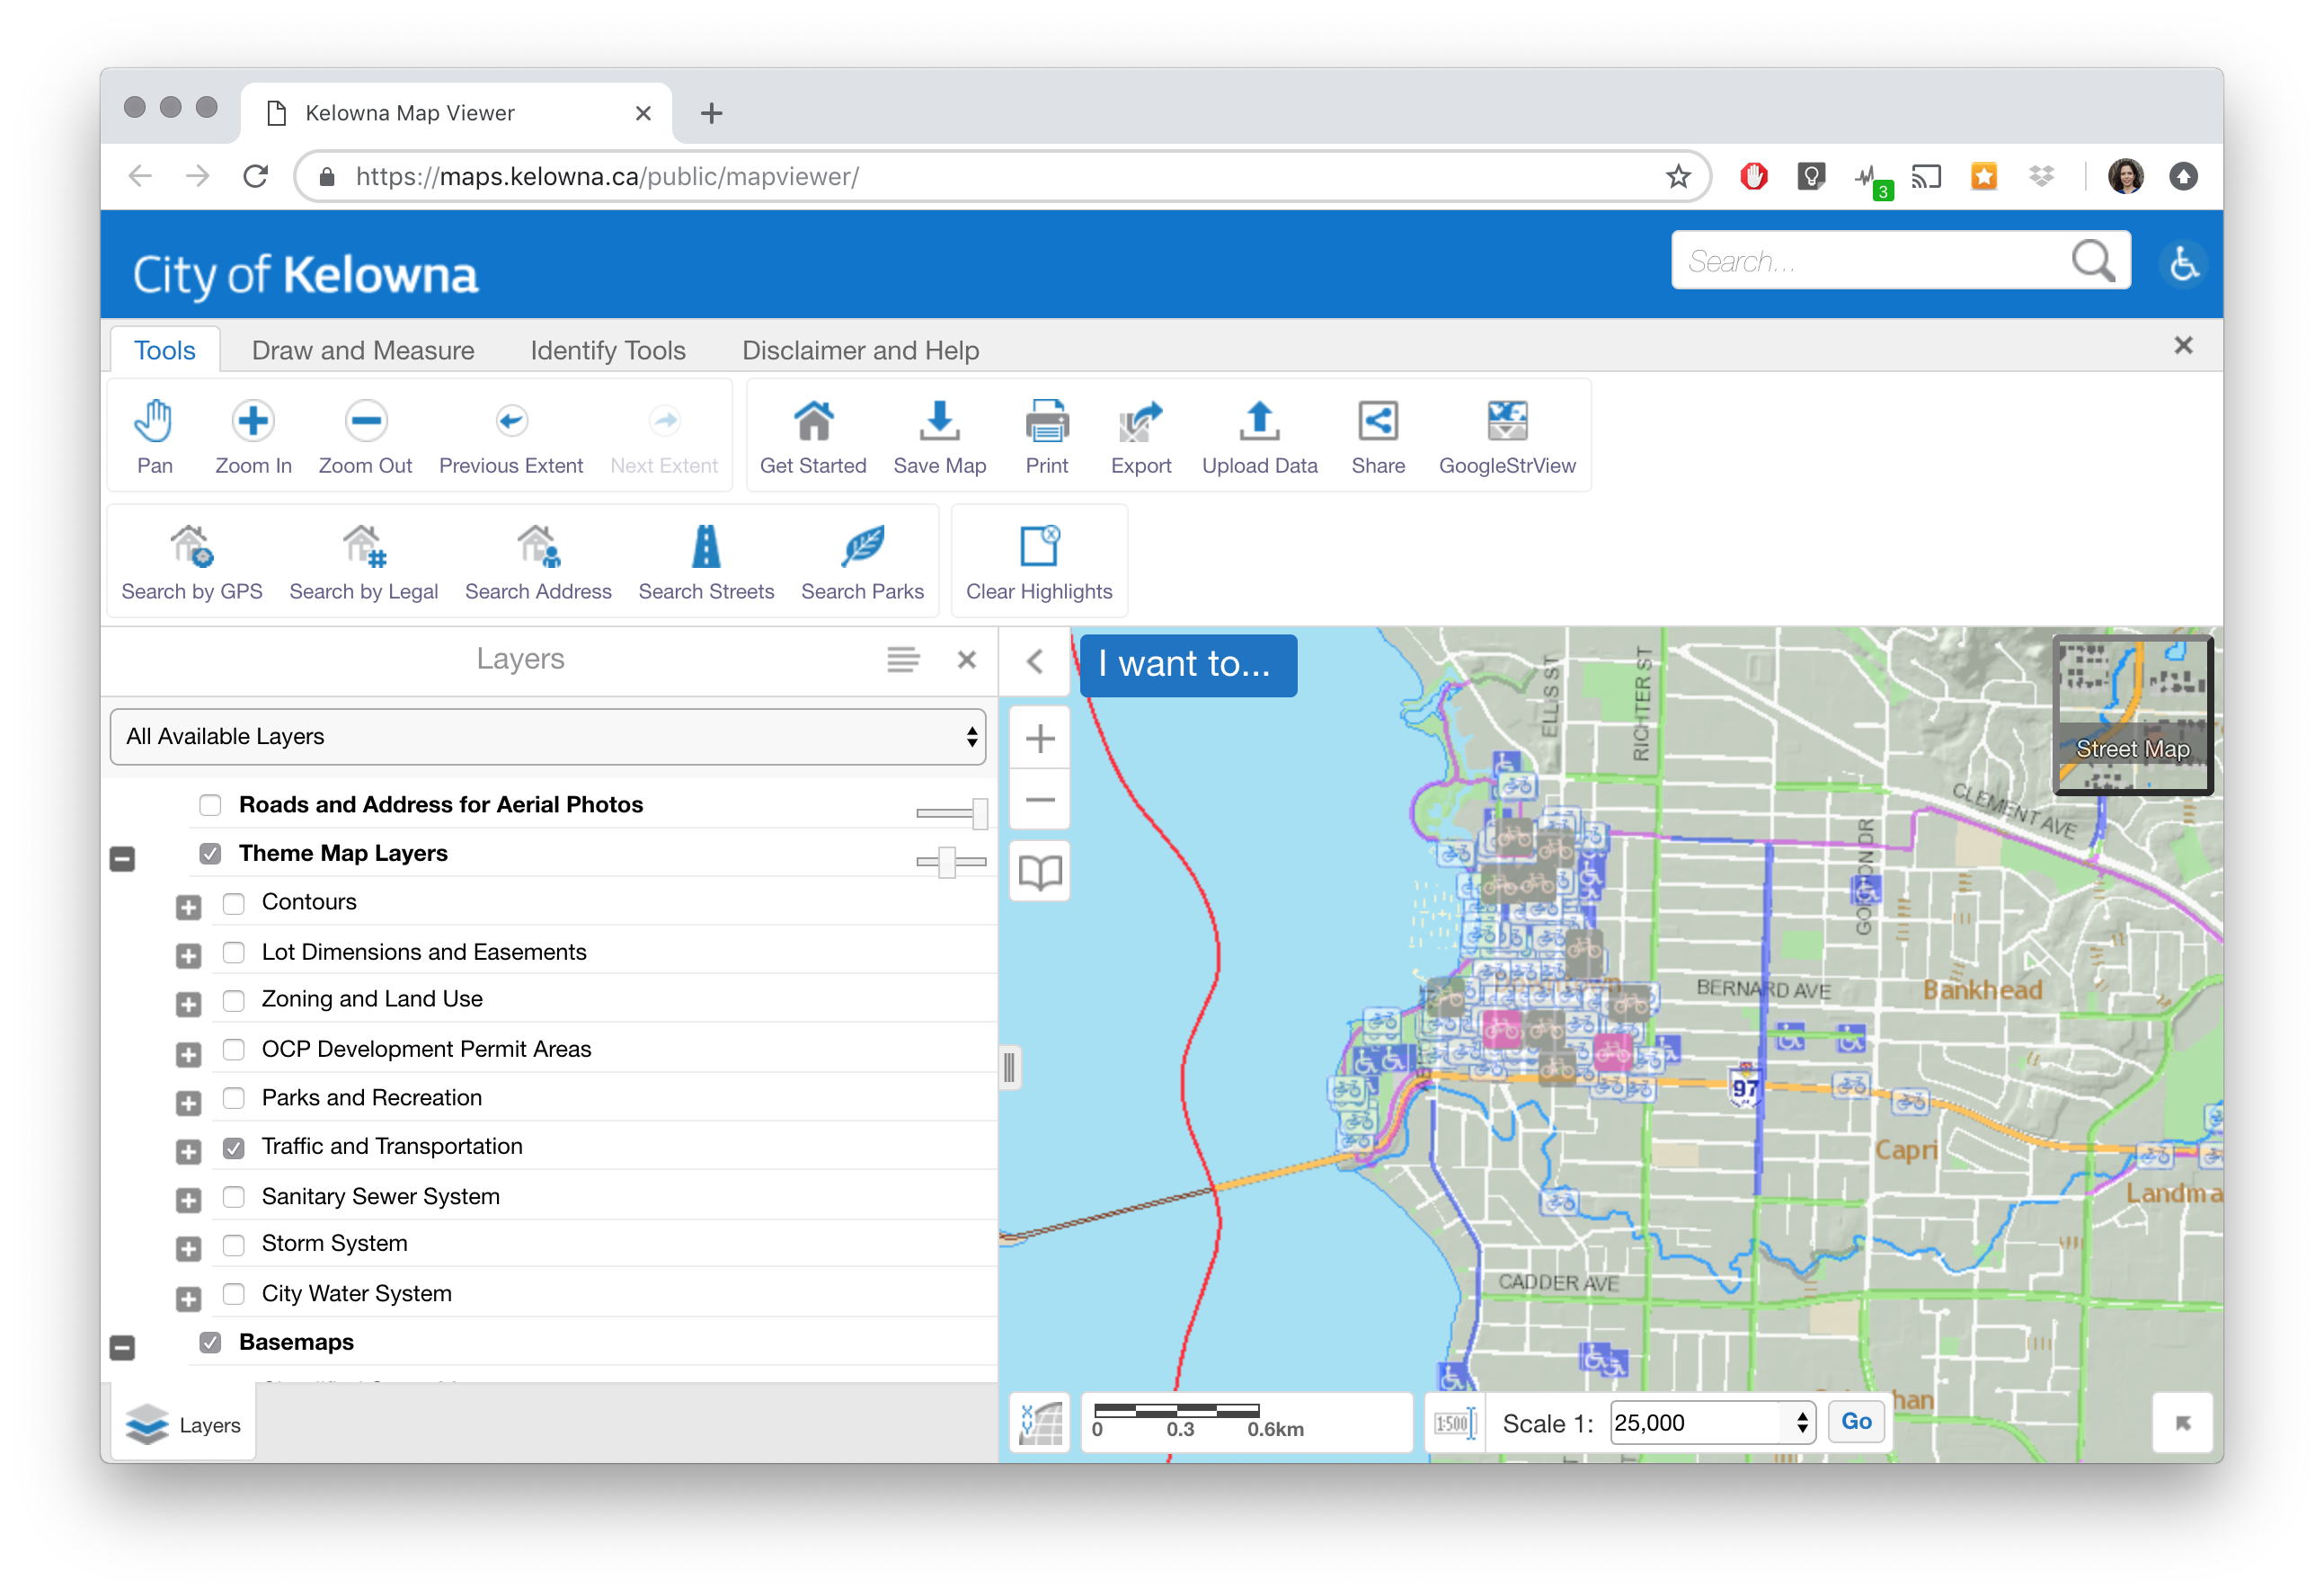
\includegraphics[width= 0.9\textwidth]{img/kelownalayers}
\end{frame}

%
%\begin{frame}
%\ft{Accessing GIS}
%GIS is available through different platforms ranging from powerful servers to cellphones. 
%\end{frame}

\begin{frame}\ft{Representing GIS data: Raster and Vector}

There are two common methods for representing GIS data.\nl

 \define{Raster representation} uses a matrix (grid of cells) of data values.
\begin{itemize}
\item useful for storing data that varies continuously, eg. a satellite image, a surface of chemical concentrations\nl
\end{itemize}


 \define{Vector representation} adds features (points, polygons) onto a map each with its own coordinates and attributes.
\begin{itemize}
\item Vector models are useful for storing data that has discrete boundaries, such as country borders, land parcels, and streets.
\end{itemize}
\end{frame}

\begin{frame}\ft{Vector Representation}
\define{Vector representation} adds features onto a map with their own coordinates and attributes.
\begin{itemize}
\item Features stored as series of x-y coordinates and may be points, lines, polygons.
\item Features are linked to a row in a data table which may have multiple attributes describing it.
\end{itemize}
Allows for very precise specification of features by coordinates which may have multiple attributes.

\end{frame}

\begin{frame}\ft{Raster Representation}
A \define{raster} stores data as a matrix of data points that is georeferenced to earth's surface.
\begin{itemize}
\item The value at each data point may be discrete (AKA thematic) or continuous.
%\item Scanned images are continuous.
\item Often used to store continuously changing values such as elevation.
\end{itemize}

Resolution measured by cell size.
\begin{itemize}
\item The level of detail  is often dependent on the cell (pixel) size, or spatial resolution.
%\item Since space is $N^2$, smaller cell sizes result in much large raster files
\item Cells must be small enough to capture adequate detail but large enough so computer storage and analysis can be performed efficiently
\item Smaller cell cells implies more detail
\item Raster formats: GRID, geoTIFF (both georeferenced), TIFF
\end{itemize}
\end{frame}

\begin{frame}
\ft{Raster vs. Vector Representation}
\begin{center}
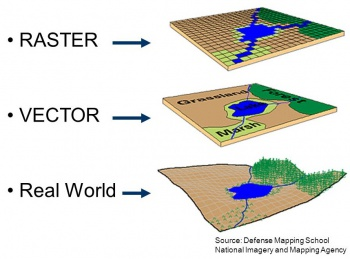
\includegraphics[width=0.75\textwidth]{img/350px-Raster_vs_Vector_a.jpg}
\end{center}
\end{frame}


\begin{frame}\ft{Raster vs. Vector Representation}

\begin{columns}[T] % align columns
\begin{column}{.48\textwidth}
Vector - \textcolor{sgreen}{Advantages}
\begin{itemize}
\item precision of coordinates
\item may have multiple attributes per feature
\item less storage space required
%\item flexible cartography
\item easier to scale
\end{itemize}
Vector - \red{Disadvantages}:
\begin{itemize}
\item  implementation of overlay operations more difficult
%\item hard to perform surface analysis
\item not easy for continuous data storage
\end{itemize}
\end{column}%
\hfill%
\begin{column}{.48\textwidth}

Raster - \textcolor{sgreen}{Advantages}:
\begin{itemize}
\item simple, robust format
\item implicit georeferencing
\item stores continuous data
%\item surface analysis, faster analysis
\item easy implementation of overlay operations
\end{itemize}

Raster -  \red{Disadvantages}:
\begin{itemize}
\item storage space
\item lower precision
\end{itemize}

\end{column}%
\end{columns}
\end{frame}


\begin{frame}
\begin{example}
Which of the following statements are TRUE?
\begin{itemize}
\item In a raster if the cell size decreases by half, the resolution increases.
%\item Rasters are often useful for scanning or remote sensing applications. 
\item A raster typically stores only one numeric data value per cell. 
\item A vector format may allow multiple attributes to describe each feature. 
\item Vector representation is better suited for continuous data than rasters.
\end{itemize}
\end{example}
\end{frame}



\begin{frame}
\begin{block}{Answer}
Which of the following statements are TRUE?
\begin{itemize}
\item In a raster if the cell size decreases by half, the resolution increases. \pcmark
%\item Rasters are often useful for scanning or remote sensing applications. \pcmark
\item A raster typically stores only one numeric data value per cell. \pcmark
\item A vector format may allow multiple attributes to describe each feature. \pcmark
\item Vector representation is better suited for continuous data than rasters.\pxmark
\end{itemize}
\end{block}
\end{frame}





\begin{frame}\ft{Representing Geographical Data}
A geographic data set requires a description of its coordinate system for display and analysis, often called the \define{spatial reference}.\nl

Components:
\begin{itemize}
\item Geographic coordinate system (GCS) / datum - for assigning coordinates to points on the earth's surface
\item Projection - for mapping 3D spherical view to 2D plane
%\item Storage units (degrees, meters, etc.)
%\item Resolution - accuracy of the measurements
\end{itemize}
\end{frame}

\begin{frame}\ft{Geographic Coordinate System}
Latitude and Longitude
\begin{center}
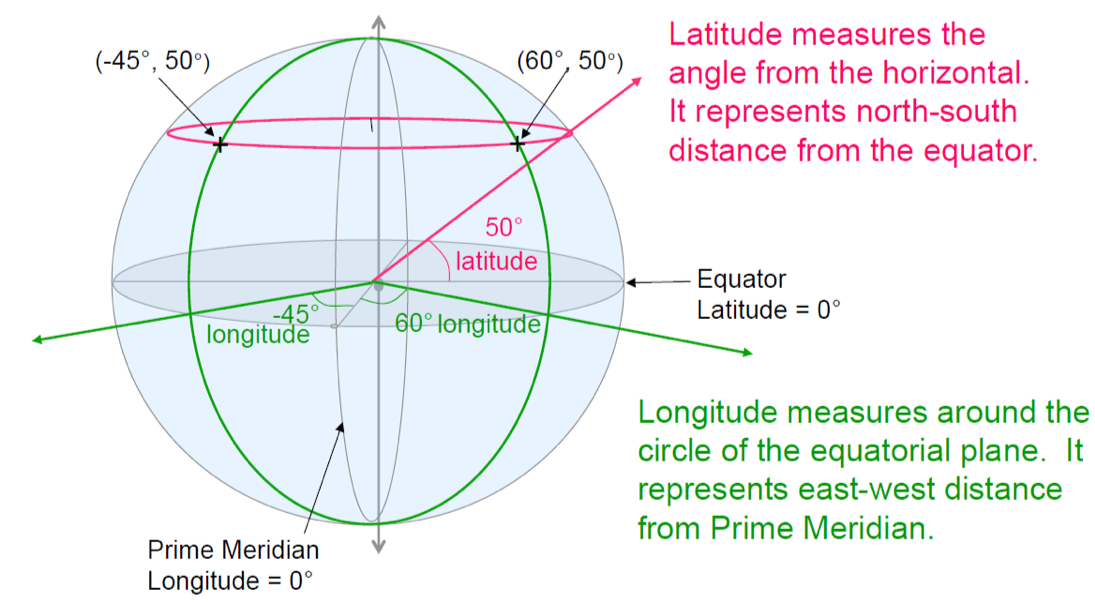
\includegraphics[width=0.8\textwidth]{img/latlong.png}
\end{center}
\end{frame}


{
\setbeamercolor{background canvas}{bg=black}
\begin{frame}\ft{GCS - Earth is not a Perfect Sphere}
\begin{center}
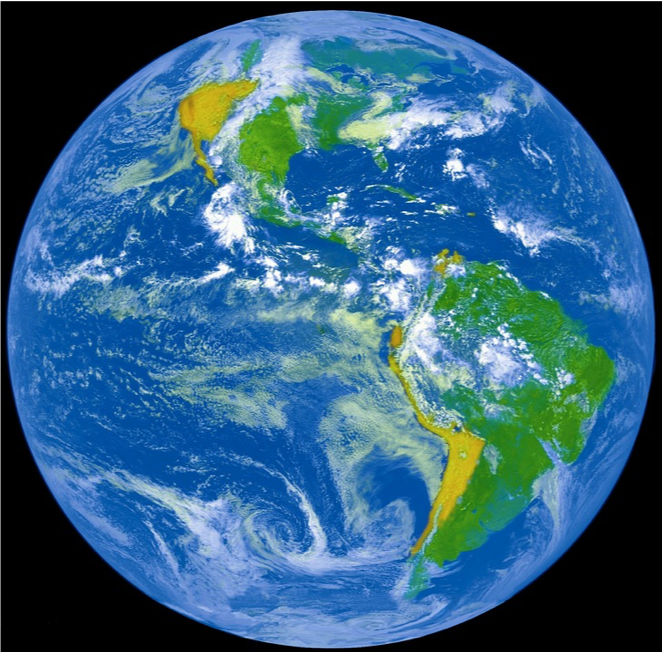
\includegraphics[width=0.44\textwidth]{img/earth1}\quad
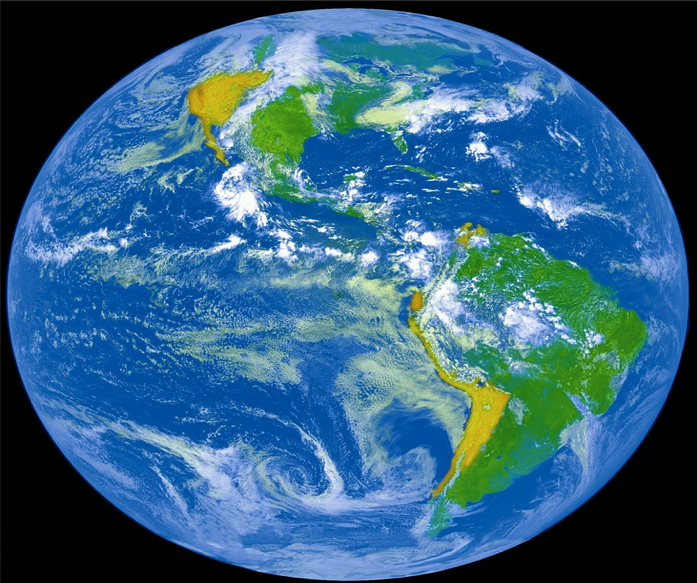
\includegraphics[width=0.44\textwidth]{img/earth2}
\end{center}
\end{frame}
}

%https://www.jmu.edu/cisr/research/sic/standards/ellipsoid.htm

\begin{frame}\ft{Earth is not a Perfect Ellipse}
\begin{columns}[T] % align columns
\begin{column}{.58\textwidth}
The earth has been approximated by various ellipsoids over time. Current standard was given in Maling, 1989.
\nl

Still not perfect as topography affects the height of surface features.\nl
A \define{geoid} is an earth model that takes into account surface height from the centre of earth. (defined by gravity measurements - see \href{https://en.wikipedia.org/wiki/Geoid}{here})
\end{column}%
\hfill%
\begin{column}{.4\textwidth}
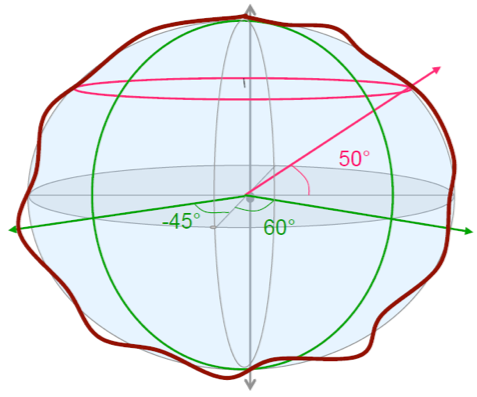
\includegraphics[width=0.9\textwidth]{img/swiggles.png}\\
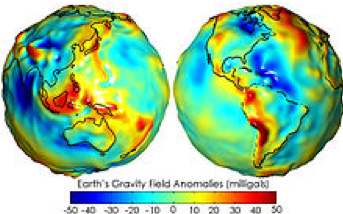
\includegraphics[width=0.9\textwidth]{img/earth3}
\end{column}%
\end{columns}
\end{frame}

\begin{frame}\ft{Datum}

A \define{datum} is a mapping to minimize the difference between geoid and ellipsoid. Shifts ellipsoid relative to geoid for a particular location.\nl

Datum components:
\begin{itemize}
\item ellipsoid used
\item adjustment or fit (translation of center)\nl
\end{itemize}

Note this means different datums are incompatible. Make sure you know your datum.
\begin{itemize}
\item  Example: WGS 84 - reference coordinate system for GPS
\end{itemize}
\end{frame}


\begin{frame}\ft{Projections}
A \define{projection} transforms a spherical coordinate system to a planar coordinate system. Each projection has different benefits and distortions.
\begin{center}
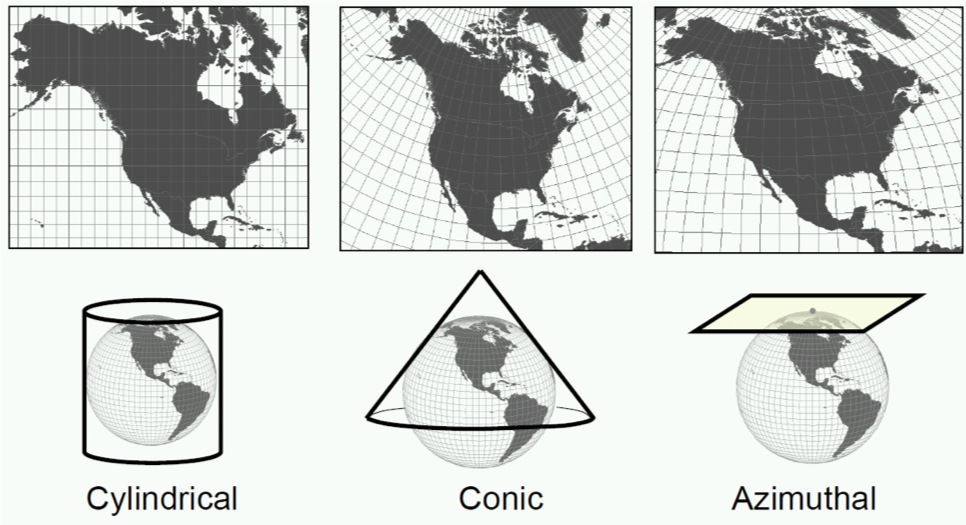
\includegraphics[width=0.9\textwidth]{img/projection.png}
\end{center}


\end{frame}





%\begin{frame}\ft{GPS data}
%
%\begin{itemize}
%\item GPS units collect points with a datum and projection. (eg. Lat-Lon NAD 1983).]\nl
%
%\item Important to record datum when perform analysis later.
%
%\end{itemize}
%\end{frame}

\begin{frame}\ft{Map Design Process}
Determine objectives
\begin{itemize}
\item Know audience and purpose, use case

\end{itemize}
Decide on data and layers required
\begin{itemize}
\item What types of data: points, line, area, volume, temporal?

\end{itemize}
Plan map layout
Choose colors and symbols
\begin{itemize}
\item Use colors consistent with understanding (red/green) and real-world
\item Use bold colors sparingly.  Color/size use strategically for emphasis.
\end{itemize}
Create!
\end{frame}


\begin{frame}
\begin{example}
Which of the following statements are TRUE?
\begin{enumerate}[A)]
\item The earth can be modeled as a perfect spheroid.
\item Latitude measures the angle from the horizontal. 
\item The zero degree for longitude is the equator.
\item A projection will cause a distortion when representing 3D as 2D. 
\item A datum consists of a mapping between a geoid and an ellipsoid.
\end{enumerate}
\end{example}
\end{frame}



\begin{frame}
\begin{block}{Answer}
Which of the following statements are TRUE?
\begin{enumerate}[A)]
\item The earth can be modeled as a perfect spheroid.\pxmark
\item Latitude measures the angle from the horizontal. \pcmark
\item The zero degree for longitude is the equator. (true for latitude, 0 degree for longitude is prime meridan)\pxmark
\item A projection will cause a distortion when representing 3D as 2D. \pcmark
\item A datum consists of a mapping between a geoid and an ellipsoid.\pcmark
\end{enumerate}
\end{block}
\end{frame}


\section{Google Maps}


\begin{frame}\ft{Google Maps}
There are a variety of GIS tools and software to use. We will use Google Maps, specifically Google My Maps, as it is easy to use and handles many of the details for us.\nl

Google My Maps Link: \url{https://www.google.com/maps/d/u/1}\nl

This uses vector representation format and layers consisting of single or groups of objects (features classes) can be easily added.\nl
Supports importing data from files, including KML, CSV, and others as well as entering data via searching or map exploring.

\end{frame}

\begin{frame}\ft{KML}
KML or Keyhole Markup Language uses XML to represent geographic information for visualization.
\begin{itemize}
\item Supported by Google and international standard in 2008.
\item KML file represents features for display on maps with latitude/longitude coordinates.
\item Data file is often in zipped form (KMZ files).
\end{itemize}
Example:

\begin{center}
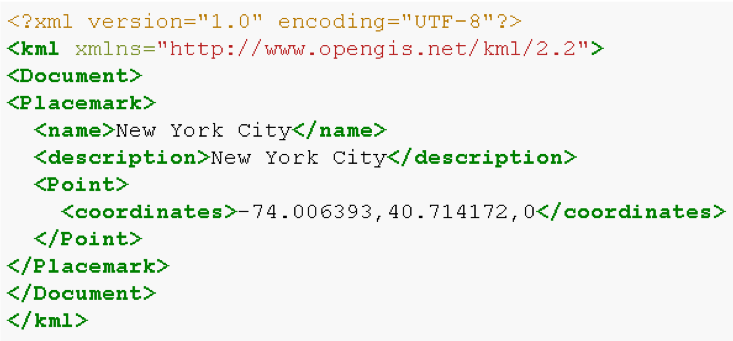
\includegraphics[width=0.8\textwidth]{xml}
\end{center}

\end{frame}




\begin{frame}\ft{Layers on google maps}
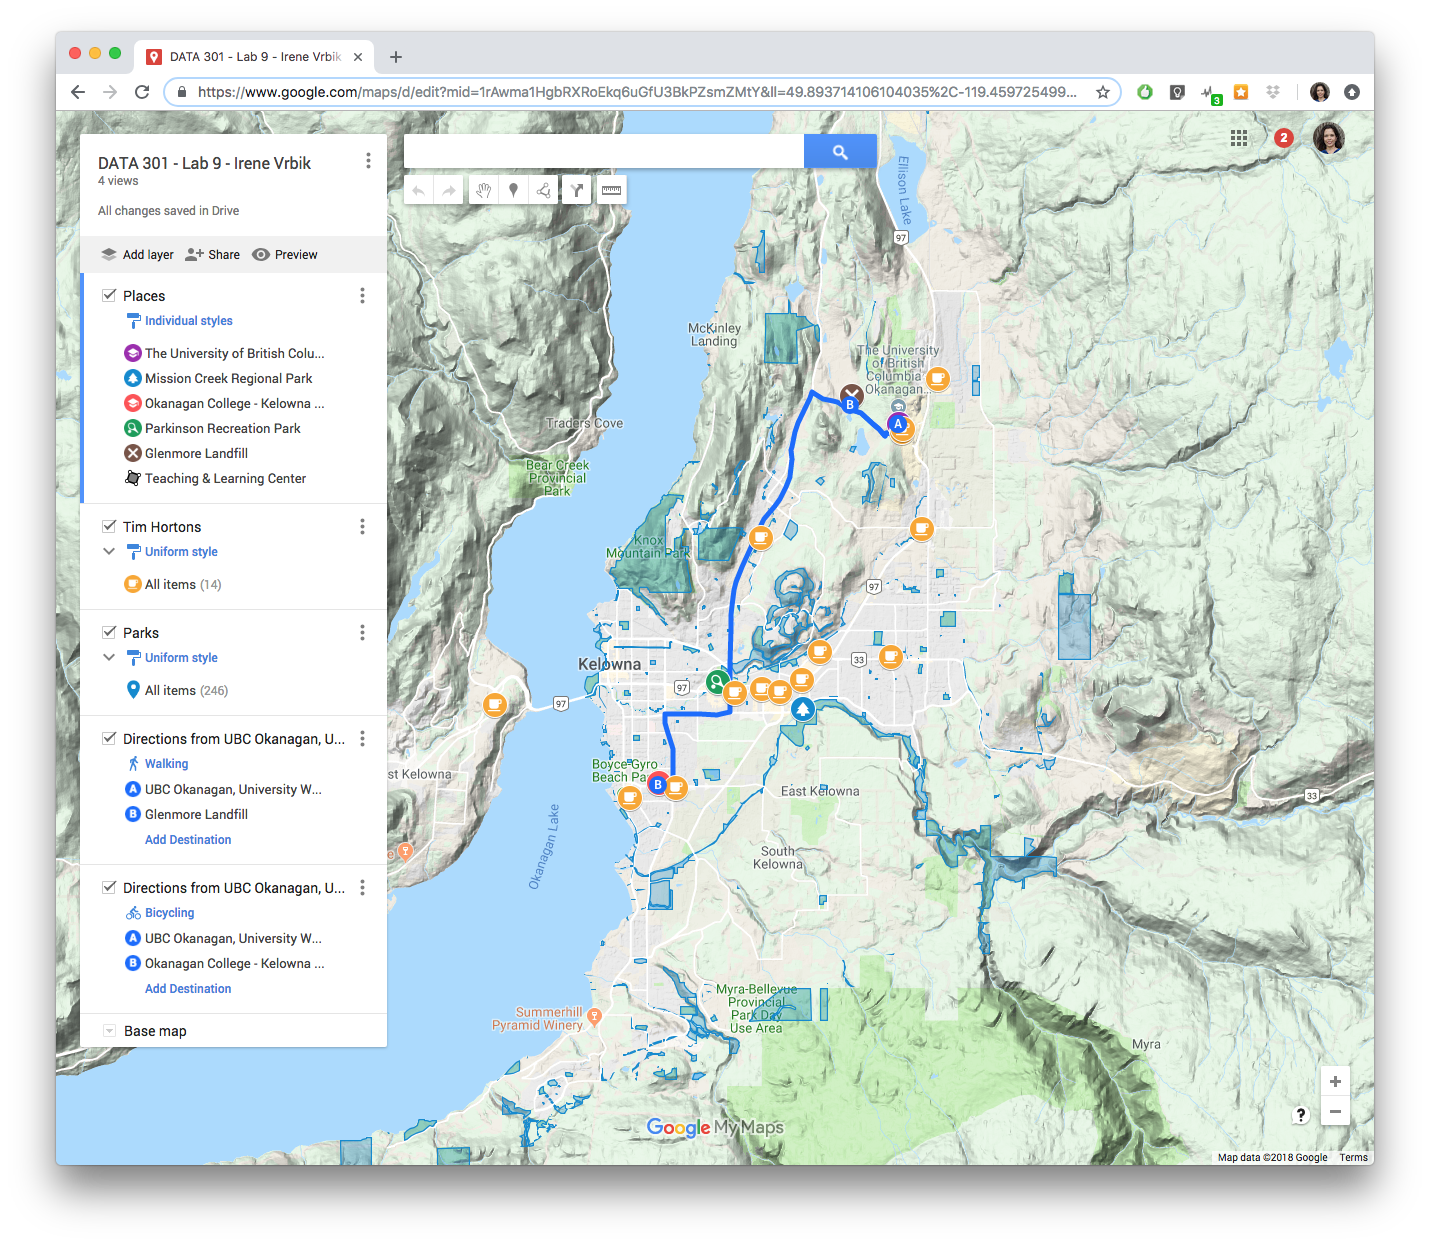
\includegraphics[width=0.8\textwidth]{googlemymaps}
\end{frame}


%\begin{frame}\ft{Try It: Google My Maps (Create your own)}
%Build a map that has the following:
%\begin{itemize}
%\item Two layers
%\item Three features per layer
%\item At least one marker with an image
%\item An area 
%\item A driving route
%\item Import an open data set, eg. \href{http://www.kelowna.ca/CM/Page3936.aspx}{City of Kelowna data} 
%\end{itemize}
%
%Suggestion: Add a map with places you have been or would like to visit.
%
%\end{frame}



\begin{frame}\ft{Google Maps API with Python}
The Google Maps API can be used with Python to access and manipulate geographical data using a Python program. 
\url{https://developers.google.com/maps/web-services/client-library}

Services and features:
\begin{itemize}
\item Geocoding and reverse geocoding
\item Directions (walking, driving, transit)
\item Distance calculations and routes
\item Elevations
\item Geolocation (based on WIFI and cell towers)
\item Road information and speed limits
\item Times zones and places (points of interest)
\end{itemize}
\end{frame}

\begin{frame}\ft{Google Maps API - Getting an API Key}
The first step is to get a API key that allows access to the Google services. This API key should be kept private and not shared!
\begin{itemize}
\item To get a key you will need a Google account.
\item For more on securing API keys see  \href{https://support.google.com/cloud/answer/6310037}{here}
\end{itemize}
N.B.  Google Maps web APIs have 25,000 free requests per day.\nl

Get an API key using Google Developer Console (get API key \href{https://developers.google.com/maps/documentation/directions/get-api-key}{here}, see 1 minute tutorial \href{https://elfsight.com/blog/2018/06/how-to-get-google-maps-api-key-guide/}{here})
\nl

With directions API, test with: 
\url{https://maps.googleapis.com/maps/api/directions/json?origin=Toronto&destination=Montreal&key=yourkey}

\red{replace \red{\tt yourkey} above!}
\end{frame}


\begin{frame}
The directions API will return your result in {\bf json} format
\begin{center}
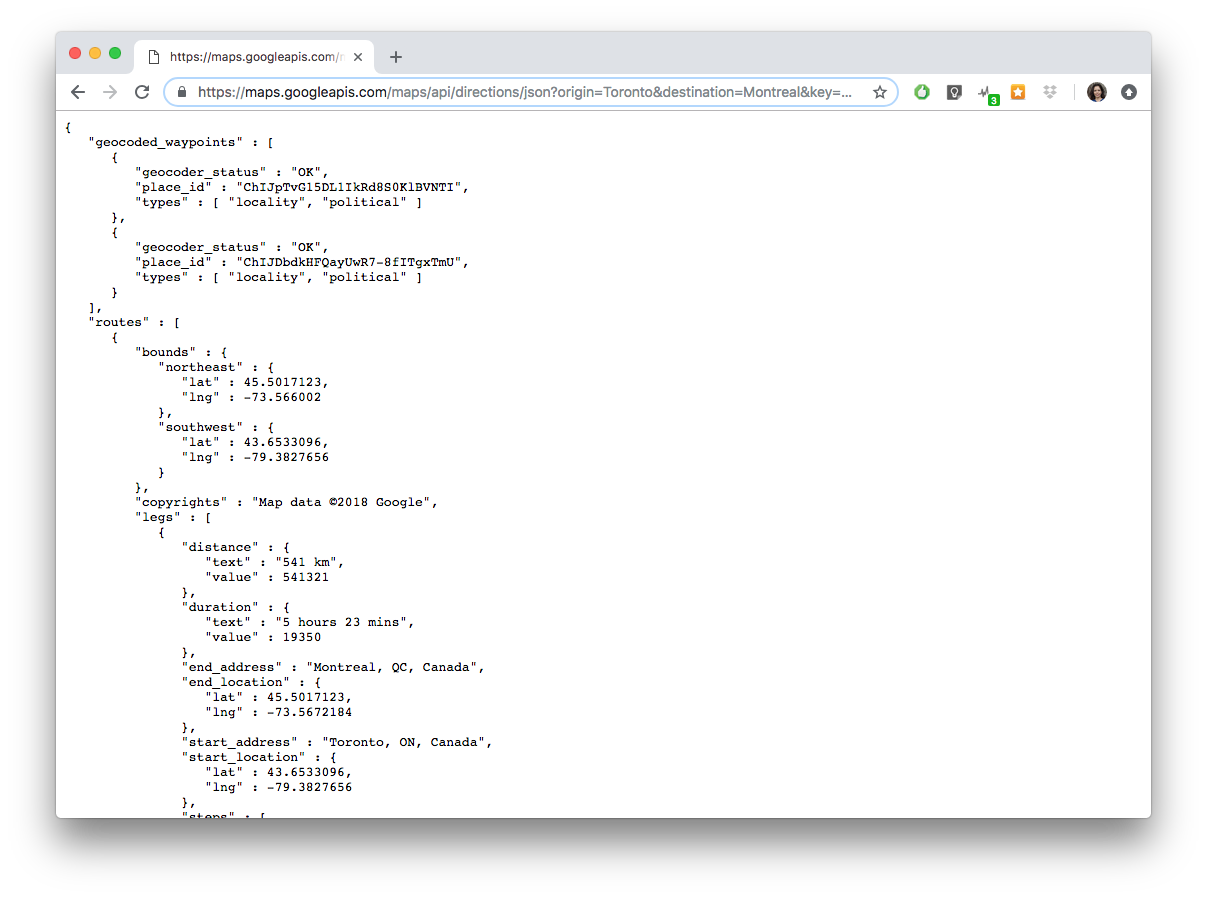
\includegraphics[width=0.99\textwidth]{img/Montreal.png}
\end{center}
\end{frame}




\begin{frame}[fragile]\ft{Google Maps and Python}
Google My Maps is an easy-to-use tool for displaying geographical information. The Google Maps API can be used with Python.\nl

We can install google maps for python using the following command:\\[0.2in]
\begin{Verbatim}[xleftmargin=2em, xrightmargin=1.5em, frame=single, label=Install google maps via command line, framesep=0.5em]
pip install -U googlemaps
\end{Verbatim}
\end{frame}

\begin{frame}
\begin{itemize}
\item One common problem when working with spatial data is going from human-understood locations to specific locations on a map.\nl
\item \define{Geocoding} is the process of converting addresses (like a street address) into geographic coordinates (like latitude and longitude), which you can use to place markers on a map, or position the map.\nl
\item This module provides an easy way to do this which uses the the \hyperlink{https://developers.google.com/maps/documentation/geocoding/start} {Geocoding API}.

\end{itemize}




\end{frame}


\begin{frame}[fragile]\ft{Python Google Maps API Example}
\begin{Verbatim}[xleftmargin=0em, xrightmargin=0em, frame=single, label=Geocoding with Python, framesep=0.5em, fontsize=\small, commandchars=\\\{\}]
import googlemaps
from datetime import datetime

# TODO: Replace <yourkey> with a valid API key. 
gmaps = googlemaps.Client(key='yourkey')

# Use \textcolor{orange}{Geocoding} API to look up latitude, longitude
address = '3333 University Way, Kelowna, BC, Canada'
geocode_result = gmaps.geocode(address)

print("Geocoding address...")
print("Address:",address, "Coordinates:",
	geocode_result[0]["geometry"]["location"])
\end{Verbatim}
\end{frame}

\begin{frame}\ft{Python Google Maps API Example}
\begin{center}
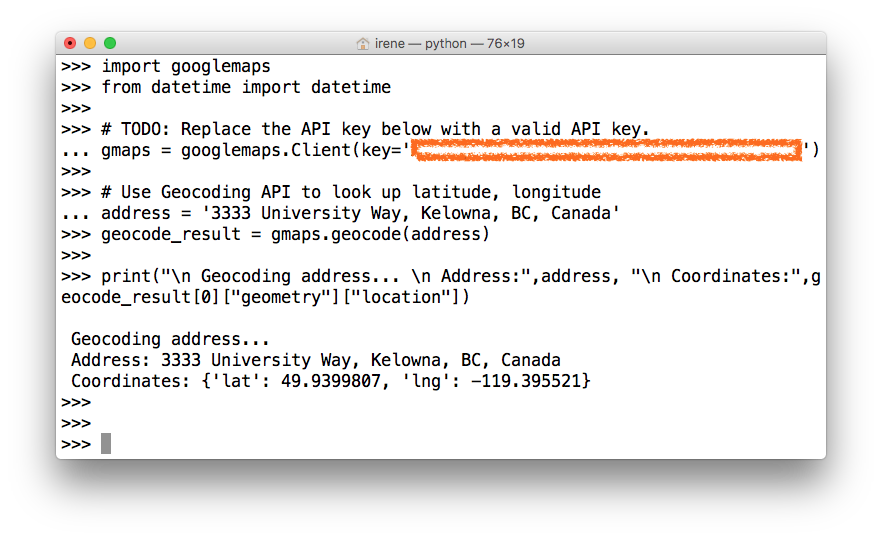
\includegraphics[width=0.9\textwidth]{georef}
\end{center}
\end{frame}


\begin{frame}[fragile]\ft{Python Google Maps API Example 2}
\begin{Verbatim}[xleftmargin=0em, xrightmargin=0em, frame=single, label=reverse geocode with python, framesep=0.5em, fontsize=\small, commandchars=\\\{\}]
# Look up an address with \textcolor{orange}{reverse geocoding} (UBC Van)
lat = 49.2683043
lon = -123.2489377
reverse_geocode_result=gmaps.reverse_geocode((lat, lon))

print("Reverse geocoding...")
print("Coordinates: ",lat,lon,"Address:", 
	reverse_geocode_result[0]["formatted_address"])


\end{Verbatim}
\end{frame}

\begin{frame}\ft{Python Google Maps API Example 2}
\define{Reverse geocoding} is the process of converting geographic coordinates into a human-readable address.
\begin{center}
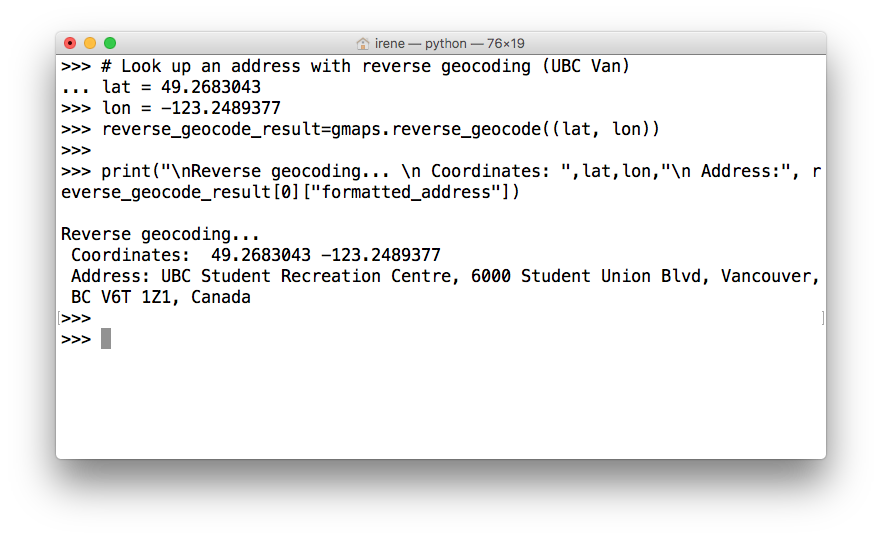
\includegraphics[width=0.9\textwidth]{reversegeo}
\end{center}
\end{frame}


\begin{frame}\ft{Python Google Maps API Example 3}
\begin{itemize}
\item The \define{Directions API} is a service that calculates directions between locations. \nl
\item You can search for directions for several modes of transportation, including transit, driving, walking, or cycling.\nl
\item Remember: we `only' have  25,000 free requests per day.\nl
\end{itemize}
\end{frame}


\begin{frame}[fragile]\ft{Python Google Maps API Example 3}
\begin{Verbatim}[xleftmargin=0em, xrightmargin=0em, frame=single, label=directions with python, framesep=0.5em, fontsize=\small, commandchars=\\\{\}]
# Request \textcolor{orange}{driving directions} between UBCO and UBCV
directions_result = gmaps.directions(address,                                      
         reverse_geocode_result[0]["formatted_address"],
         mode="driving", departure_time=datetime.now())
leg = directions_result[0]['legs'][0]

print("Driving directions...")
print("Start address:",leg['start_address'], 
      "Destination address:",leg['end_address'])
print("Distance:",leg['distance']['text'], 
      "Time:",leg['duration']['text'])

for step in leg['steps']:
    print("Step:",step['duration']['text'], 
           step['html_instructions'])

\end{Verbatim}
\end{frame}

\begin{frame}\ft{Python Google Maps API Example 3}
%The 
%\define{Directions API} is a service that calculates directions between locations. You can search for directions for several modes of transportation, including transit, driving, walking, or cycling.
\begin{center}
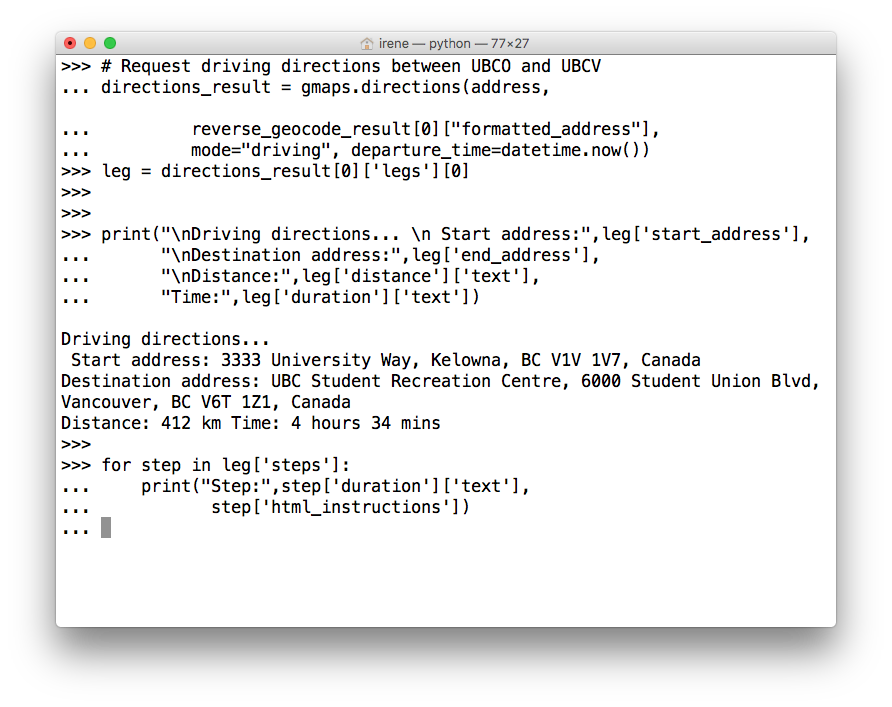
\includegraphics[width=0.9\textwidth]{drivingdir}
\end{center}
\end{frame}


\begin{frame}\ft{Python Google Maps API Example 3}
\begin{center}
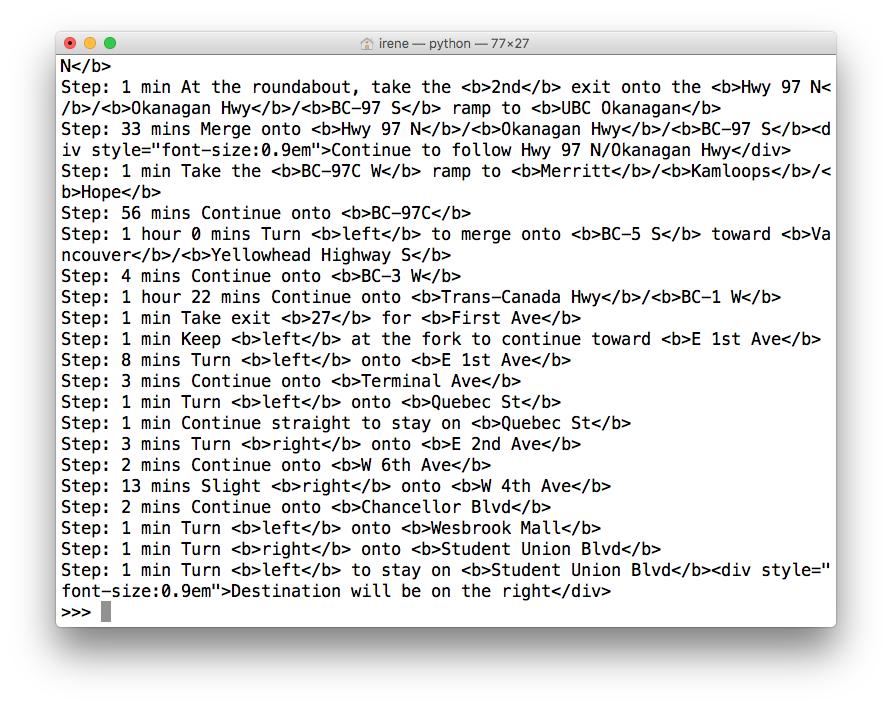
\includegraphics[width=0.9\textwidth]{drivingdir2}
\end{center}
\end{frame}

%https://www.gislounge.com/john-snows-cholera-map-gis-data/

\begin{frame}{John Snow Example}
\begin{itemize}
\item When could we use this? \nl
\item Lets consider the data analysis preformed by John Snow:
\begin{center}
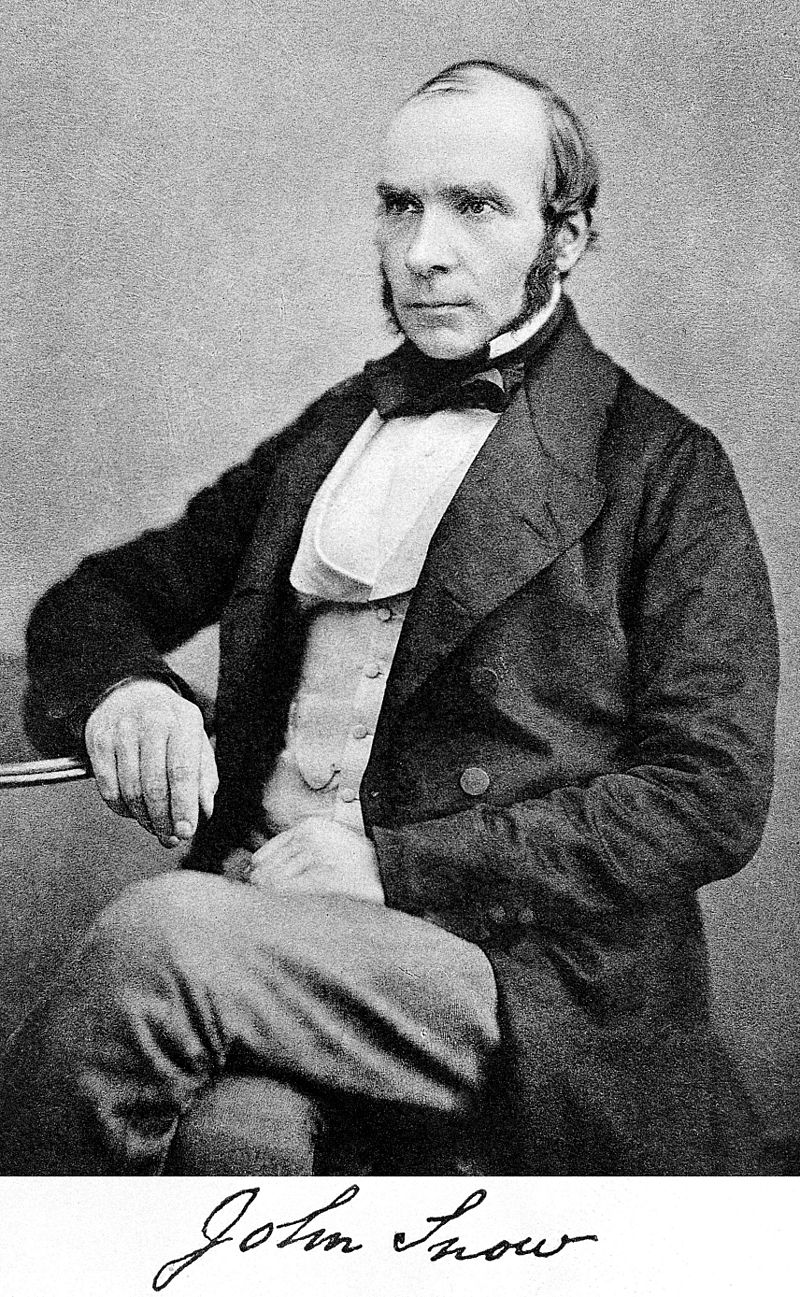
\includegraphics[height=0.65\textheight]{img/johnsnow.jpg}

\includegraphics[height=0.65\textheight]{img/jonsnow.jpg}
\end{center}
\item (not to be confused with Jon Snow from GoT)
\end{itemize}
\end{frame}

\begin{frame}\label{map}
\begin{itemize}
%\item John Snow�s well known cholera map is often cited as one of the earliest known examples of using geographic inquiry to understand a health epidemic. 
\item John Snow (March 1813 --- June 1858) was was an English physician considered to be one of the fathers of modern epidemiology.\medskip
\item He is cited as one of the earliest known examples of using GIS by famously tracing the source of a cholera outbreak in Soho, London, in 1854.\medskip
\item This outbreak took the lives of 127 people in only three days, killing over 500 by by September 10, 1854.\medskip
 \item The map on the following page is the original showing the clusters of cholera cases in the London epidemic.  \href{https://en.wikipedia.org/wiki/John_Snow}{Image source: Wikipedia}.
\end{itemize}
\end{frame}


\begin{frame}
\begin{center}
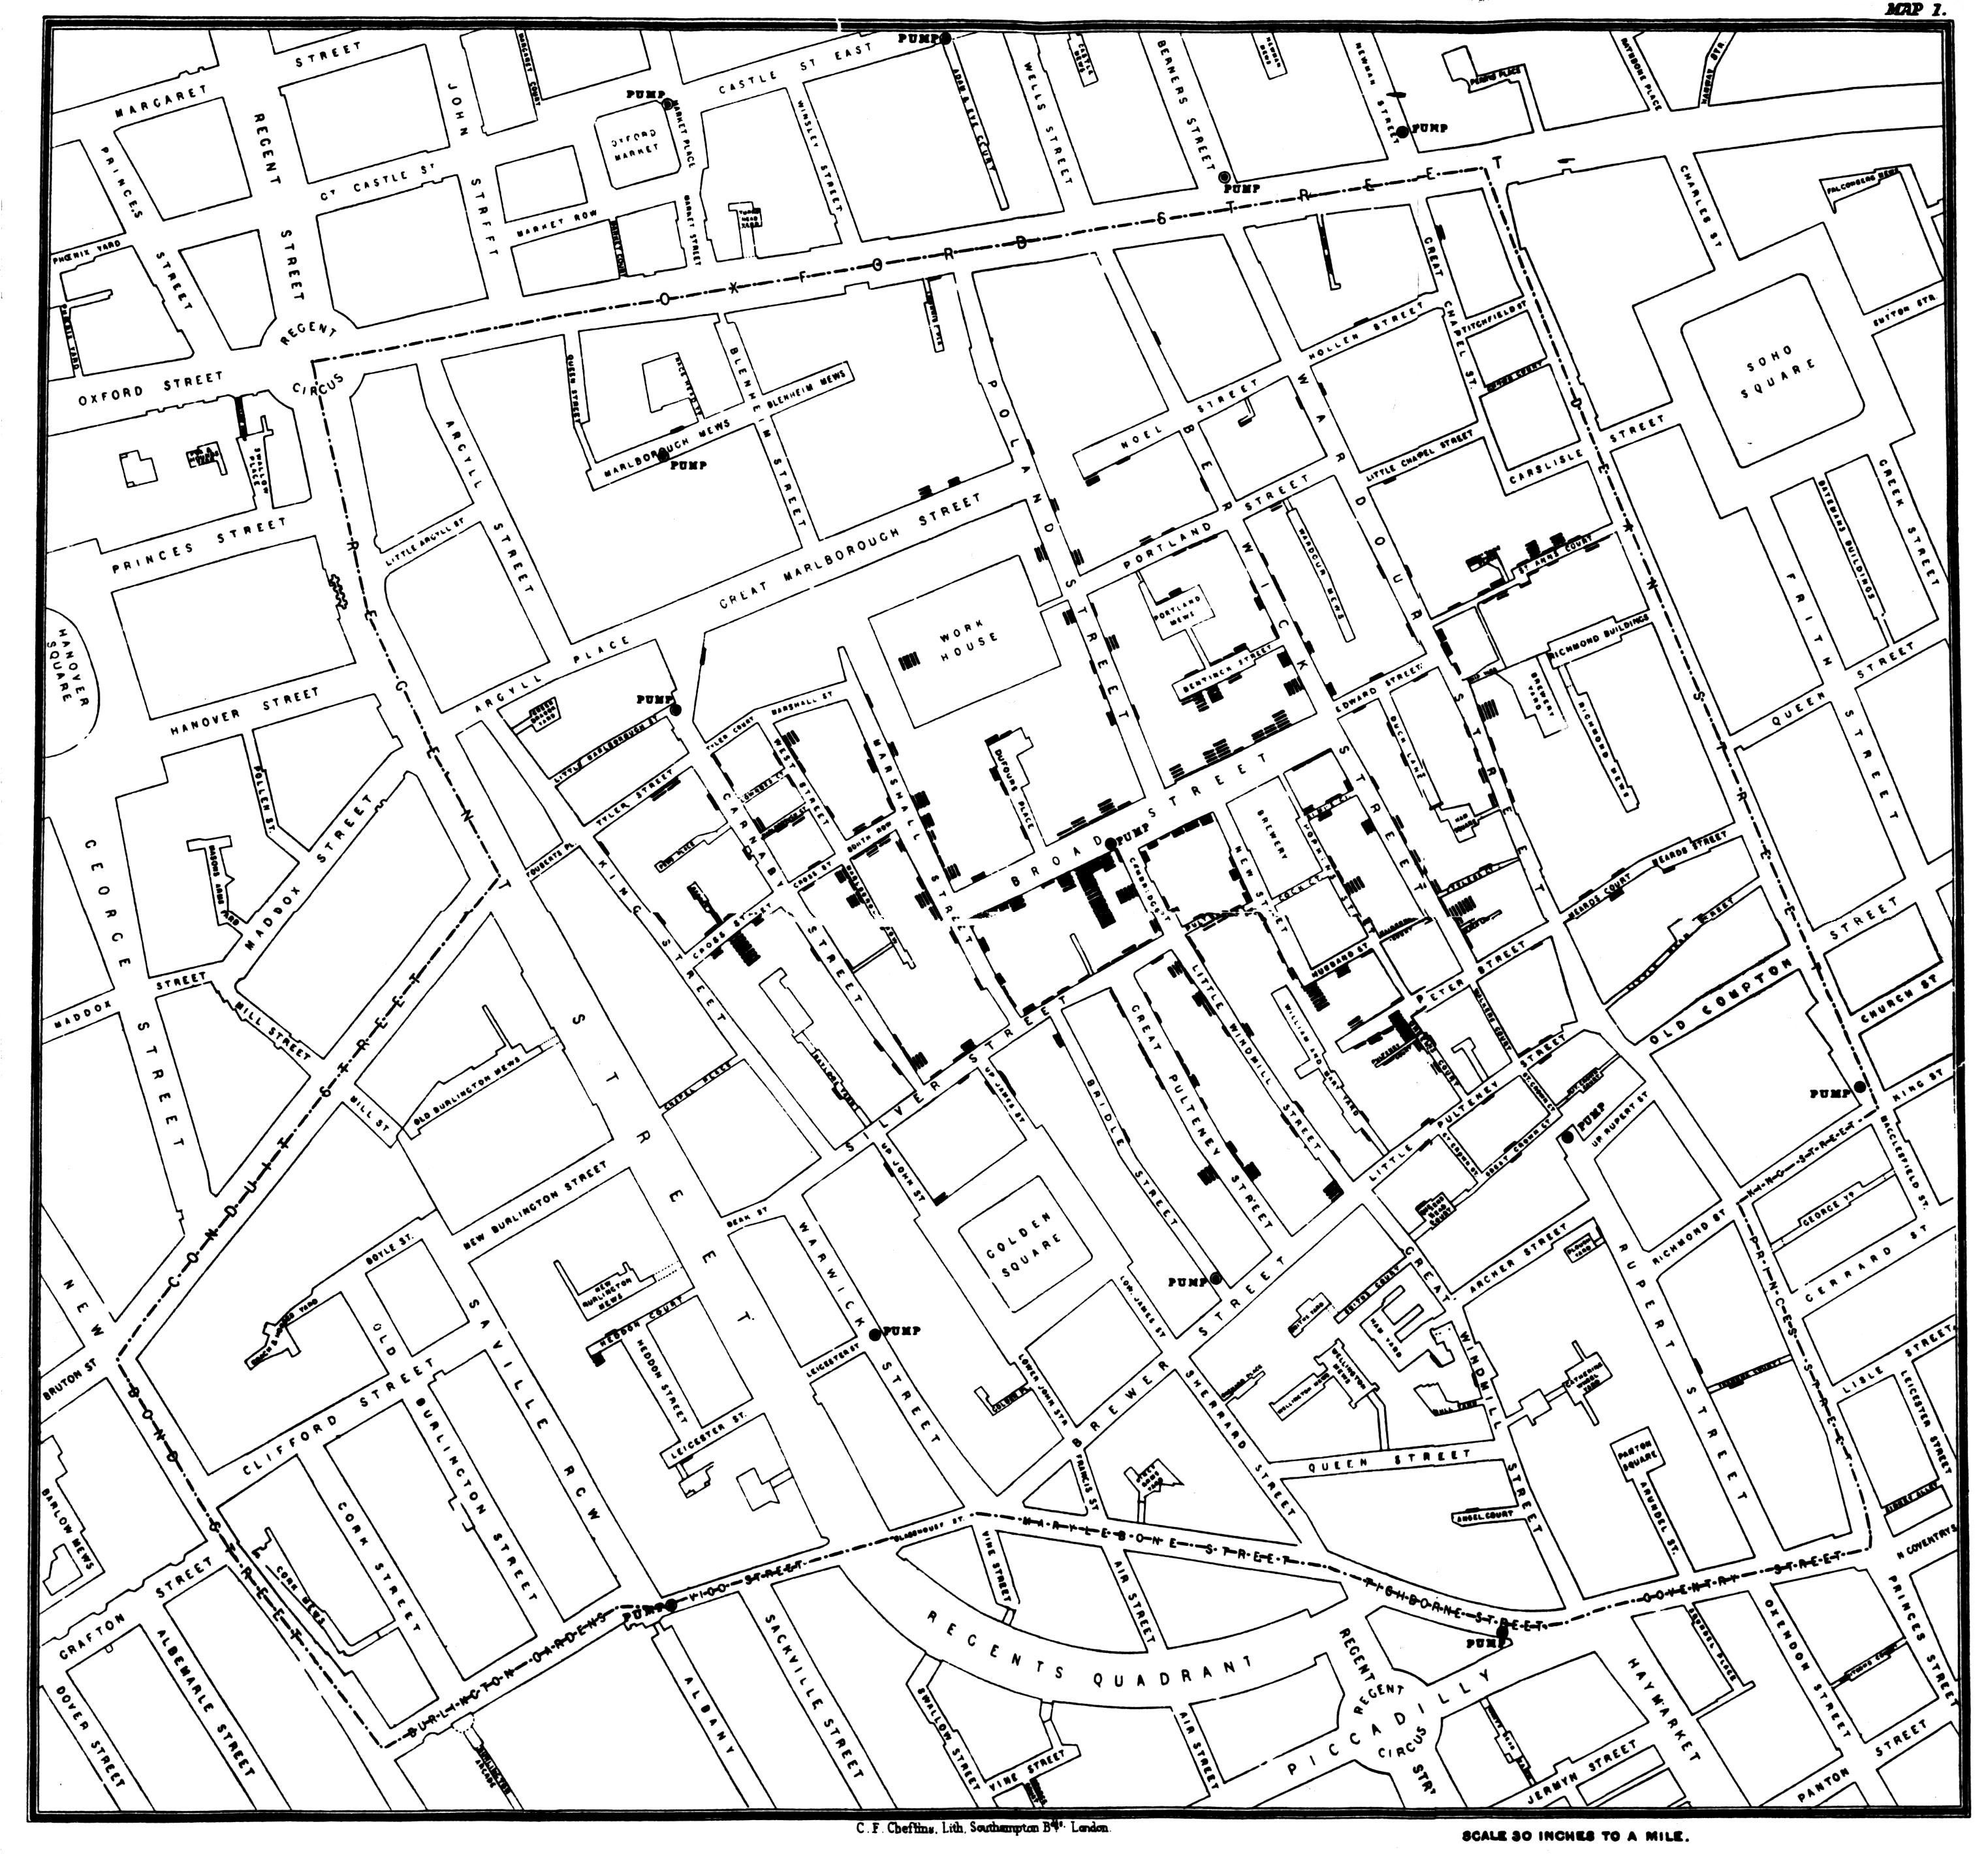
\includegraphics[width=0.8\textwidth]{img/JSmap.jpg}
\end{center}
\end{frame}

\begin{frame}
\begin{itemize}
\item Perhaps made more clear in an updated version of this map, on the following page, is that these outbreaks were clustered around the water pump on Broad Street. \nl
\item By observing these these outbreaks spatially on his \hyperlink{map}{original map}, Snow was able to form his hypothesis that a contaminated  water wells was the lead contributor to the cholera death count.\nl
\item Subsequently, Snow convince the local council to remove the handle to prevent its use.
\end{itemize}
\end{frame}

\begin{frame}{}
Image created by Robin Wilson of Southampton University: \href{http://blog.rtwilson.com/john-snows-famous-cholera-analysis-data-in-modern-gis-formats/}{source}
\begin{center}
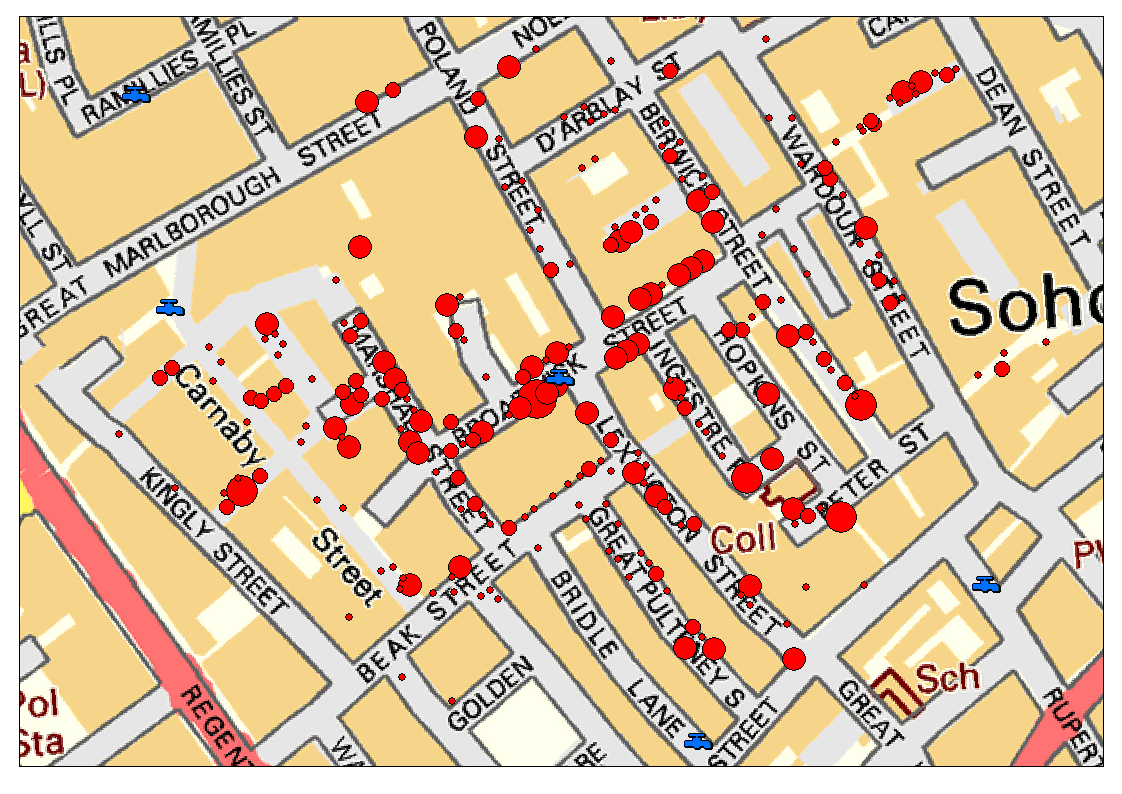
\includegraphics[width=0.8\textwidth]{img/JSmap2}
\end{center}
\end{frame}




\begin{frame}\ft{Conclusion}
\emph{Geographic Information Systems} are systems designed for storing, manipulating, analyzing, and displaying spatial and geographical data.
A GIS supports:

\begin{itemize}
\item importing data from various sources in different formats
\item organizing the data into layers or groups and integrating data from sources
\item displaying the data visually as maps or 3D visualizations to help interpret the data
\end{itemize}
Understanding how GIS data is encoded using a geographical coordinate system and datums is important when interpreting and combining data from sources.\nl
Google My Maps is an easy-to-use tool for displaying geographical information. The Google Maps API can be used with Python.


\end{frame}


\begin{frame}\ft{Obejectives}
\begin{itemize}
\item Provide examples where a GIS is used
\item Define GIS and list some of its features/components
\item Appreciate history of GIS including Canadian connection
\item List and use GIS features: text, point, line, polygon
\item Explain the relationship between features, coordinates, and attributes
\item Provide an example on how interval and categorical data is displayed
\item Define: scale, precision, resolution and perform simple calculations
\item Define: feature class, layer
\item Compare and contrast raster versus vector representations
\end{itemize}

\end{frame}



\begin{frame}\ft{Obejectives}
\begin{itemize}
\item Define and use latitude and longitude
\item Explain the challenge in modeling a point on the earth's surface given that it is not a perfect sphere and has topography
\item Explain role and connection between a geoid, spheroid, datum

\item Explain the purpose of a projection and understand different projections have different benefits and distortions
\item Apply a map design process to produce visually appealing maps
\item Define and use KML
\item Create a map with Google My Maps with various features
\item Write a program to access the Google Maps API using Python

\end{itemize}

\end{frame}













\end{document}

